\section{Aprendizaje Profundo (Deep Learning)}

El Aprendizaje Profundo (\textit{Deep Learning}) es un subcampo especializado del Aprendizaje Automático, fundamentado en el uso de Redes Neuronales Artificiales (ANN) con múltiples capas ocultas. 

Mientras que los algoritmos clásicos de \textit{Machine Learning} alcanzan una asíntota de rendimiento independientemente de la cantidad de datos que se les proporcione, los modelos de aprendizaje profundo tienen la capacidad de continuar mejorando su precisión y escalabilidad a medida que aumenta el volumen de información y la capacidad de cómputo.

\subsection{1. La Diferencia Clave: Aprendizaje de Representaciones}
En el \textit{Machine Learning} tradicional, el rendimiento del modelo depende en gran medida de la \textbf{Ingeniería de Características} (\textit{Feature Engineering}). Un experto humano debe extraer manualmente las variables matemáticas o estadísticas más relevantes de los datos crudos antes de pasarlos al algoritmo clasificador.

El Aprendizaje Profundo elimina este cuello de botella mediante el \textbf{Aprendizaje de Representaciones} (\textit{Representation Learning}). La red neuronal procesa los datos crudos (como matrices de píxeles en una imagen o secuencias temporales) y descubre automáticamente las características más relevantes de forma jerárquica a través de sus capas.

\subsection{2. Estructura Matemática Fundamental}
Una Red Neuronal Profunda (DNN) puede modelarse como una composición de funciones matemáticas no lineales. Para una capa arbitraria $l$ en una red de $L$ capas, la transformación afín aplicada a la matriz de activaciones de la capa anterior $A^{[l-1]}$, seguida de una función de activación, se define rigurosamente de la siguiente manera:

\begin{equation}
    Z^{[l]} = W^{[l]} A^{[l-1]} + b^{[l]}
\end{equation}
\begin{equation}
    A^{[l]} = \sigma^{[l]}(Z^{[l]})
\end{equation}

Donde:
\begin{itemize}
    \item $W^{[l]}$ es la matriz de pesos de dimensión $(n^{[l]}, n^{[l-1]})$.
    \item $b^{[l]}$ es el vector de sesgos (\textit{bias}) de dimensión $(n^{[l]}, 1)$.
    \item $Z^{[l]}$ es la transformación lineal previa a la activación.
    \item $\sigma^{[l]}$ es la función de activación no lineal, dependiente y diferenciable (e.g., ReLU, Sigmoide, o Tangente Hiperbólica).
\end{itemize}

El modelo predictivo final es la composición completa de estas $L$ transformaciones matriciales sucesivas, evaluada desde la entrada original $X$ (que equivale a $A^{[0]}$) hasta generar la matriz de salida final $\hat{Y} = A^{[L]}$.

\subsection{3. Representación Gráfica: ML Clásico vs. Deep Learning}
El siguiente esquema ilustra cómo el Aprendizaje Profundo unifica las etapas de representación y clasificación en un único flujo de optimización continua (entrenamiento \textit{end-to-end}).

\begin{figure}[H]
    \centering
    \shorthandoff{>} % Prevenir errores con babel
    \resizebox{\textwidth}{!}{%
    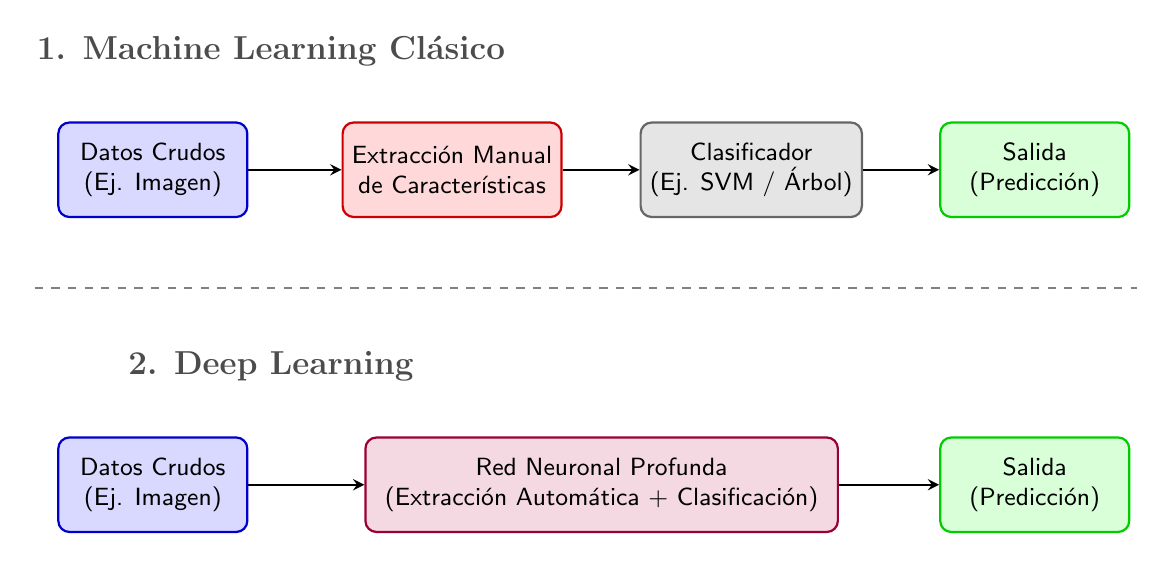
\begin{tikzpicture}[
        box/.style = {rectangle, rounded corners, draw=black, thick, minimum width=2.4cm, minimum height=1.2cm, align=center, font=\small\sffamily},
        input/.style = {box, fill=blue!15, draw=blue!80!black},
        manual/.style = {box, fill=red!15, draw=red!80!black},
        auto/.style = {box, fill=purple!15, draw=purple!80!black},
        model/.style = {box, fill=gray!20, draw=gray!80!black},
        output/.style = {box, fill=green!15, draw=green!80!black},
        arrow/.style = {thick, ->, >=stealth}
    ]
    % ================= PARTE SUPERIOR: ML CLÁSICO =================
    \node[font=\large\bfseries, text=black!70, align=left] at (1.5, 1.5) {1. Machine Learning Clásico};
    %
    \node[input] (in1) at (0, 0) {Datos Crudos \\ (Ej. Imagen)};
    \node[manual] (feat1) at (3.8, 0) {Extracción Manual \\ de Características};
    \node[model] (clas1) at (7.6, 0) {Clasificador \\ (Ej. SVM / Árbol)};
    \node[output] (out1) at (11.2, 0) {Salida \\ (Predicción)};
    %
    \draw[arrow] (in1) -- (feat1);
    \draw[arrow] (feat1) -- (clas1);
    \draw[arrow] (clas1) -- (out1);

    % Línea separadora
    \draw[dashed, thick, gray] (-1.5, -1.5) -- (12.5, -1.5);

    % ================= PARTE INFERIOR: DEEP LEARNING =================
    \node[font=\large\bfseries, text=black!70, align=left] at (1.5, -2.5) {2. Deep Learning};
    %
    \node[input] (in2) at (0, -4) {Datos Crudos \\ (Ej. Imagen)};
    \node[auto, minimum width=6cm] (dl) at (5.7, -4) {Red Neuronal Profunda \\ (Extracción Automática + Clasificación)};
    \node[output] (out2) at (11.2, -4) {Salida \\ (Predicción)};
    %
    \draw[arrow] (in2) -- (dl);
    \draw[arrow] (dl) -- (out2);

    \end{tikzpicture}%
    }
    \caption{Diferencia en el flujo de trabajo: El Aprendizaje Profundo elimina la dependencia de la ingeniería manual de características, delegando a la red neuronal tanto la extracción de representaciones como la decisión final.}
    \label{fig:ml_vs_dl}
\end{figure}